\chapter{Bayesian Inference}
\label{chap:bay}
%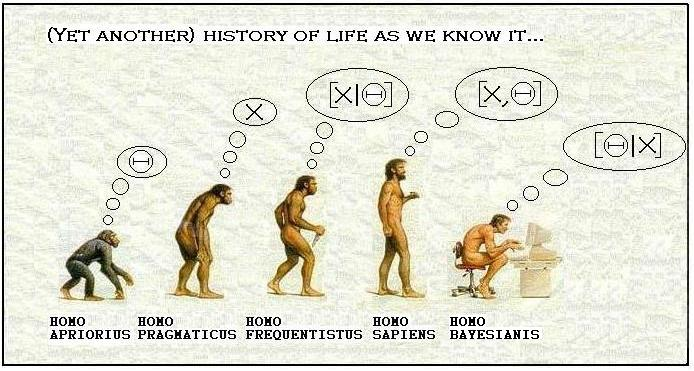
\includegraphics[width=\textwidth]{bayesian_evol}

\epigraph{We anticipate the sun will rise tomorrow, not just because it has always done so far, but because this is predicted by {\em models}, which accord with {\em data}. Any perceived failure of the sun to rise would more likely be a hallucination.}{\davidmackay{}}

%  * BRIEF intro to difference between bayesian and frequentist, and the nature of probability
%      - Continuous vs. Discrete
%      - Aleatoric vs. Epistemological \davidspiegelhalter
%
%  * Parameter estimation and model comparison
%       -Example? (e.g.\ coin flipping, --- anything better?)
%
%  * Sampling as method for describing high-dimensional probability distributions.
%      - MH as good technique
%      - Need for evidences


Science is not the search for truth. Instead, scientists concern themselves with the construction of models. These models have their relative merit determined using data.\footnote{The opening statement of this chapter was in fact the first thing \rafiblumenfeld{} said to us for our part IB Physics supervisions.}

% Mathematics -- if then, conditional truth
% Science -- weaker: observations -> possibilities 

\section{Probability}
\label{sec:bay:prob}

Probability is the mathematical language of uncertainty. It is a methodology of assigning a numerical weighting to outcomes or {\em events}. An event is any subset of the sample space $\Omega$. Some examples of discrete and continuous sample spaces are:
\begin{enumerate}
  \item The outcome of a coin flip $\Omega_1=\{\mathrm{Heads},\mathrm{Tails}\}$.
  \item The measured position of an electron $\Omega_2=\mathbb{R}$.
\end{enumerate}
For example, an event could be that the electrons position $x$ is measured to be $-1<x<0.5$. The role of probability is to assign a weighting to all subsets, which roughly corresponds to the ``chance'' that such an event would occur. Probability should therefore be additive:
\begin{equation}
  A,B \mathrm{\ disjoint} \Rightarrow \Prob{A \cup B} = \Prob{A} + \Prob{B}.
  \label{eqn:bay:add}
\end{equation}
One also normalises the probability distribution so that $\Prob{\Omega} = 1$. The above is effectively a paraphrasing of Kolmogorov's axioms of probability.

%In addition, if one has two disjoint sample spaces, for example $\Omega_1$ and $\Omega_2$ mentioned above, one may combine these into a single samples space ${\Omega=\Omega_1\otimes\Omega_2}$, then probability should be multiplicative.





This entire section may be summarised succinctly and formally as:
\begin{quote}
  Probability is any additive mapping $\mathrm{P}$ from the power set $2^\Omega$ of the sample space $\Omega$ to $[0,1]\in \mathbb{R}$, such that $\Prob{\Omega}=1$.
\end{quote}
\johnskilling{} has derived probability from measurement-theoretical grounds\citep[chap. 1]{Bayesian_methods_in_cosmology}, which provides a more intuitive backing to the definition.



\section{Bayesian vs.\ Frequentist}
\label{sec:bay:bayesian_frequentist}

Whilst the previous section outlined the properties that probability must satisfy, it has not detailed how one should assign probability. Indeed, we have merely referred to probability as a measure of ``chance'', but declined to define what this means.

There are two fundamental types of probability: {\em Aleatoric\/} and {\em Epistemological}. Aleatoric systems are genuinely random, for example: the flip of a coin, or the click on a Geiger counter. Epistemological probability governs systems where the randomness is associated with a subjective lack of knowledge. For example, before prince George was born, bookmakers took bets on whether William and Kate's baby was a boy or a girl. 

The Frequentist school of thought defines probability as:
\begin{description}
  \item[Frequentist Probability:]``The limiting relative frequency of an event.''
\end{description}
I.e.\ if a coin has $\Prob{\mathrm{Head}}=\frac{1}{2}$, then if you were to toss it an arbitrarily large number of times, the fraction of times one would get closer and closer to $\frac{1}{2}$. This is the version of probability that most people encounter early in their mathematical education, but it has several issues.

This definition applies relatively well to Aleatoric systems (since an experiment can often be run a large number of times). However, for epistemological systems, it is all but useless. The frequentist solution is therefore to disregard the latter kind of probability.

Most people's experiences with probability will likely involve betting scenarios, such as William and Kate's baby. Here it is obvious that the betting odds should be approximately $1:1$,\footnote{Betting odds of $a:b$ against indicates a probability of success of $\frac{b}{a+b}$.}\footnote{In fact the probability of a boy being conceived across the population is roughly 51\%, in order to biologically account for male infant mortality. An individual's probability of conceiving a boy or a girl will vary from person to person and in time.}\footnote{A good bookmaker will obviously take this into account, and give you slightly worse odds in order to ensure their profit.} but it should be also be clear that these odds most certainly do not refer to an event that can be repeated an arbitrarily large number of times.

The alternative definition of probability is {\em Bayesian\/}:
\begin{description}
  \item[Bayesian Probability:] ``A degree of belief that an event will occur.'' 
\end{description}
Note that Bayesian probability is {\em subjective}, it matters who's degree of belief one is considering. Probabilities are assigned only with a given state of knowledge. Effectively, Bayesians place aleatoric and epistemological probability under the same umbrella. 

Pure mathematics deals in relative truth or falsity, i.e.\ given initial assumptions, all statements are assigned to the set $\{F,T\}\equiv\{0,1\}$. Bayesian probability can be thought of as a blurring of this process, namely from initial assumptions, various conclusions are assigned a number from the continuum between $[0,1]$.

\section{Parameter Estimation \& Model Comparison}
\label{sec:bay:model_comp}
The typical problem of science is the construction of a model $\model$ in order to explain some dataset $\data$. 


\section{An example: biased coins}
For example, assume that you toss a coin $N=20$ times, and observe a dataset of $\data = 16$ heads. Is this enough to cause us to doubt the fairness of the coin?

The standard model $\model_0$ is that a coin toss consists of a binomial trial with probability $\frac{1}{2}$. Elementary probability tells us that the chance of getting this data is:
\begin{equation}
  \Probc{\data}{\model_0}= {^{N}C_\data} {\left( \frac{1}{2} \right)}^{N}  = 4.6\times 10^{-3}.
  \label{eqn:bay:M0}
\end{equation}
Note that as should be expected, the chance of obtaining this exact dataset is small. 

If we allow for the possibility that the coin could be any probability $p$, we can encapsulate this in a second model $\model_1$.
\begin{equation}
  \Probc{\data}{p,\model_1}= {^{N}C_\data}\: {p}^{\data} {\left(1 - p \right)}^{N-\data} 
  \label{eqn:bay:M1}
\end{equation}
This second model is not ideal, since we haven't specified the parameter $p$. If we choose $p=\frac{1}{2}$ we recover $\model_0$. It is tempting to choose $p$ such that the probability of getting the data is maximised. This would be an example of a {\em maximum likelihood\/} approach. In this case, the method indicates\footnote{Proof left as exercise to the reader.} we should choose $p = \frac{\data}{N}$. 

Maximum likelihood has its drawbacks, particularly in the case of a low volume of data. After $N=1$ toss, it seems a little premature to choose either $p=1$ or $p=0$ depending on whether we see a head or a tail. Instead picking a specific value of $p$, one could instead ``spread your bets'' and consider several different values of $p$. The full generalisation of this is to consider a continuum of models, and define an initial probability distribution $\Probc{p}{\model_1}$. These can be interpreted as our initial assumptions on the value of $p$, or our initial degree of belief in its value
A natural assumption is to try and be as unbiased as possible and assume that $p$ is equally likely to take any value in between $0$ and $1$. We therefore have:
\begin{equation}
  \Probc{p}{\model_1}=\left\{
  \begin{array}{lr}
    1 &:0\le p\le1\\
    0 &:\text{otherwise.}\\
  \end{array}
  \right.\label{eqn:bay:prior1}
\end{equation}
With this distribution, we can work out what the overall probability of obtaining the dataset $\data$ is, by marginalising over all values of $p$:
\begin{align}
  \Probc{\data}{\model_1} 
  &= \int \Probc{\data}{p,\model_1}\Probc{p}{\model_1}\: dp \\
  &= \int_0^1 {^{N}C_\data}\: {p}^{\data} {\left(1 - p \right)}^{N-\data}\: dp \\
  &= \frac{1}{n+1} = 4.8\times10^{-2}
  \label{eqn:bay:marg}
\end{align}
This is quite telling, because our initial choice for $\Probc{p}{\model_1}$~(\ref{eqn:bay:prior1}) indicates that we expect all data sets with equal probability (independent of $\data$). This is therefore a ``minimally suspicious'' choice in spread.

We now have two equations~(\ref{eqn:bay:M0})~\&~(\ref{eqn:bay:marg}) which detail the probability of getting the dataset $\data$ given the choice of model. However, what we are really after is the probability of the model, given the dataset $\Probc{\model}{\data}$. To compute this, we use Bayes' theorem
\begin{equation}
  \Probc{\model}{\data} = \frac{\Probc{\data}{\model}\Prob{\model}}{\Prob{\data}}.
  \label{eqn:bay:bay_md}
\end{equation}
In order to complete the calculation, we must assign a probability to each model. A natural choice is to consider $\Prob{\model_0}=\Prob{\model_1}=\frac{1}{2}$. $\Prob{\data}$ is just a normalising constant, computed as:
\begin{equation}
  \Prob{\data} = \sum_i \Probc{\data}{\model_i}\Prob{\model_i}, 
  \label{eqn:bay:norm}
\end{equation}
so we may finally compute
\begin{equation}
  \Probc{\model_0}{\data} = 0.088 \qquad
  \Probc{\model_1}{\data} = 0.922
  \label{eqn:bay:comp}
\end{equation}
In other words, a betting man would put money on $\model_1$ with odds of $10:1$ for. Another way of thinking of this is that $\model_1$ is ten times better at describing the data than $\model_0$.

$\model_1$ can go further however. We may also use Bayes' theorem to compute 
\begin{equation}
  \Probc{p}{\data,\model_1} = \frac{\Probc{\data}{p,\model_1}\Probc{p}{\model_1}}{\Probc{\data}{\model_1}}.
  \label{eqn:bay:bay_p}
\end{equation}





\subsection{Nomenclature}
\label{sec:pc:nomenclature}
Scientific theory is concerned with the construction of predictive models in the context of some dataset $\data$.
A typical model $\model$ contains a set of variable parameters $\params_\model$. One may use $\model$ to calculate the probability of observing the data given a specific parameter choice:
\begin{equation}
  \Probc{\data}{\params_\model,\model}\equiv\lik.
  \label{eqn:pc:lik_def}
\end{equation}
This distribution on $\data$ is termed the {\em likelihood\/} $\lik$. From a Bayesian standpoint a model must also specify our initial degree of belief on the parameters $\params_\model$:
\begin{equation}
  \Probc{\params_\model}{\model} \equiv \prior,
  \label{eqn:pc:prior_def}
\end{equation}
This distribution on $\params_\model$ is termed the {\em prior\/} $\prior$. Typically this is a parametric distribution which quantifies our initial assumptions on the scale and spread of the parameters\footnote{Common examples include a uniform distribution between two bounds, or a Gaussian distribution with specified mean and variance.}.

The likelihood~(\ref{eqn:pc:lik_def}) is conditioned on a set of chosen values for the model parameters $\params_\model$. One may marginalise out the dependence on $\params_\model$ by integrating over the prior distribution:
\begin{equation}
  \Probc{\data}{\model} \equiv \ev = \int  \Probc{\data}{\params_\model,\model}\Probc{\params_\model}{\model}\:d\params_\model.
  \label{eqn:pc:ev_int}
\end{equation}
This quantity is termed the {\em evidence\/} $\ev$, or {\em marginalised likelihood}, and gives the probability of observing the data $\data$, conditioned on the model $\model$. Suppressing explicit dependence on the model, the evidence computation can be written as:
\begin{equation}
  \ev = \int \lik(\params)\prior(\params)\:d\params.
  \label{eqn:pc:evidence}
\end{equation}

\subsection{Parameter estimation}
\label{sec:pc:param_est}

If the prior has been specified, Bayes theorem allows us to invert the conditioning in equation~(\ref{eqn:pc:lik_def}) and find the {\em posterior\/} $\posterior$ by combining the likelihood, prior and evidence:
%
\begin{equation}
  \Probc{\params_\model}{\data,\model} = \frac{\Probc{\data}{\params_\model,\model} \Probc{\params_\model}{\model}}{\Probc{\data}{\model}},
  \label{eqn:pc:bayes_theorem}
\end{equation}
%
which is schematically written as:
\begin{equation}
  \posterior = \frac{\lik \times \pi }{\ev }.
  \label{eqn:pc:bayes_theorem_abbrv}
\end{equation}
This describes how our initial knowledge $\prior$ of the parameters updates to $\posterior$ in light of the data $\data$.
Calculation of the posterior $\posterior(\theta)$ is the domain of {\em parameter estimation}, and in high dimensions is best performed by sampling the space with a Markov-Chain Monte-Carlo approach (MCMC). Examples include Metropolis-Hastings, Gibbs sampling and Slice sampling. For the most part, the evidence $\ev$ is ignored during such calculations, and one works with an unnormalised posterior ${\posterior\propto\lik\times\prior}$.

\subsection{Model comparison}
\label{sec:pc:model_comp}

Of equal importance in scientific investigation is {\em model comparison}. Typically one has multiple competing models ${\{\model_1,\model_2,\cdots\}}$, each with their own parameters and assumptions. The data $\data$ are able to decide on the relative merits of each of these models via Bayes theorem:
\begin{align}
  \Probc{\model_i}{\data} &= \frac{\Probc{\data}{\model_i}\Prob{\model_i}}{\Prob{\data}}, \\
  &= \frac{\ev_i\pi_i}{\sum_j \ev_j\pi_j}.
\end{align}
In contrast to parameter estimation, the evidences of each model $\ev_i$ take the leading role in model comparison. One typically will choose uniform priors on the models, ${\pi_i\equiv\Prob{\model_i}= \mathrm{const}}$, and then choose to use the model with the highest evidence. However, when evidences are similar in magnitude, the correct Bayesian approach is to make inferences by marginalising over all models considered. If there is a common derived parameter $y$, with marginalised posterior $\Probc{y}{\data,\model_i}$ then one may produce the fully marginalised posterior:
\begin{equation}
  \Probc{y}{\data} = \frac{\sum_i\Probc{y}{\data,\model_i}\ev_i\pi_i}{\sum_j\ev_j\pi_j}.
\end{equation}
This fully Bayesian approach has been historically under utilised due to the difficulties in computing the evidence numerically from the integral~(\ref{eqn:pc:evidence}).


\section{Sampling}
\label{sec:bay:samp}


\begin{figure}
  \centerline{%
    \def\firstcircle{(-0.75,0) circle (1.5)}
\def\secondcircle{(0.75,0) circle (1.5)}

\begin{tikzpicture}
  \draw \firstcircle;
  \draw \secondcircle;
  \draw (-3,-2) rectangle (3,2);

  \begin{scope}
    \fill[blue!30!white] \firstcircle;
    \clip \secondcircle;
  \end{scope}

  \begin{scope}
    \clip \firstcircle;
    \fill[blue!60!white] \secondcircle;
  \end{scope}

  \draw[above left] node at (-1,0) {\(A\)};
  \draw[above right] node at (1,0) {\(B\)};
  \draw[below ] node at (0,0) {\(A\cap B\)};
  \draw[below left] node at (3,2) {\(\Omega\)};


\end{tikzpicture}


  }
  \caption{Beer-mat mathematics. This diagram is how \edjaynes{} explained Bayes' theorem to a young \stevegull{}. Out of the entire sample space $\Omega$, if we observe $A$ to be true (blue region), then the probability of $B$ given that we know $A$ is simply $\Prob{A\cap B}/\Prob{A}$. Bayes' theorem then follows by rearrangement and symmetry.}
\end{figure}


From this definition, it is useful to define conditional probability via:
\begin{equation}
  \Probc{B}{A} = \frac{\Prob{A\cap B}}{\Prob{A}}.
  \label{eqn:bay:cond}
\end{equation}
Multiplying both sides by $\Prob{A}$, and noting the symmetrical alternative:
\begin{equation}
  \Probc{B}{A}\Prob{A} = \Prob{A\cap B} = \Probc{A}{B}\Prob{B},
  \label{eqn:bay:sym}
\end{equation}
one may then derive Bayes' theorem:
\begin{align}
  \Probc{B}{A} &= \frac{\Probc{A}{B}\Prob{B}}{\Prob{A}}.\\
  \label{eqn:bay:bayes}
  \tag{Bayes' Theorem}
\end{align}




